%%%%%%%%%%%%%%%%%%%%%%%%%%%%%%%%%%%%%%%%%%%%%%%%%%%%%%%%%%%%%%%%%%%%%%%%%%
 %																		%
 %	Plantilla Latex para presentación del proyecto de curso				%
 %	Programación de Aplicaciones para Internet y la Nube					%
 %																		%
 %	Creada por: Duván Pardo, Wilson López								%
 %																		%
 %	Versión: 0.2															%
 %	Dapardoc@gmail.com ; Wilrilo@gmail.com								%
 %																		% 
 %	Se requieren los archivos  plantilla.bbl								% 
 %													%  
 %																		%
%%%%%%%%%%%%%%%%%%%%%%%%%%%%%%%%%%%%%%%%%%%%%%%%%%%%%%%%%%%%%%%%%%%%%%%%%%

\documentclass[10pt]{article}   			% Describe el tipo de documento, y el tamaño de la letra del texto

\usepackage[utf8]{inputenc}				% Define codificación para que permita caracteres latinos (acentos)
\usepackage[spanish,activeacute]{babel} 	% Paquete para poder escribir con tildes y otros caracteres especiales

\usepackage{vmargin}						% Código para margenes y formato de página
\setpapersize{A4}
\setmargins	{2.2cm}     					% margen izquierdo
			{1 cm}                 		% margen superior
			{16.5cm}               		% anchura del texto
			{23.42cm}             		% altura del texto
			{20pt}                		% altura de los encabezados
			{1.2cm}               		% espacio entre el texto y los encabezados
			{0pt}                		% altura del pie de página
			{2cm}                 		% espacio entre el texto y el pie de página

\usepackage{amsmath}						% paquete para expresiones matemáticas
\usepackage{amsfonts}					% paquete para escritura de ecuaciones 
\usepackage{amssymb}						% paquete para caracteres especiales para ecuaciones 

\usepackage{fancyhdr}					% Temas para encabezado y pie de pagina
\usepackage{fancyvrb}
\pagestyle{fancy} 

\pagenumbering{arabic} 					% Numeración de paginas {arabic roman}
\usepackage{hyperref}					% Para hipervinculos
\usepackage{graphicx}					% Para incluir imágenes
\usepackage{caption}						% Descripciones de las figuras
\usepackage{subcaption}					% Descripción varias imagenes en usa sola figura
\graphicspath{ {Imagenes/} }				% Directorio de imágenes esta capeta va donde esta el archivo tex


\usepackage{color, colortbl}				% Colores para tablas
\usepackage{listings}					% Para el código Fuente
\usepackage{xcolor}						% para color en codigos o listrings
\definecolor{limegreen}{RGB}{50,100,50}	% Definición de colores ejemplo verde en RGB
\definecolor{Red}{RGB}{220,120,120}		% se definen colores para la tabla en el cronograma pueden ser RGB 0-255 o rgb 0-1 cada componente
\definecolor{LightCyan}{rgb}{0.88,1,1}
\definecolor{azul}{RGB}{120,120,210}
\lstdefinestyle{base}{
	language=C,
	emptylines=1,
	breaklines=true,
	showspaces=fasle,
	showstringspaces=false,
	extendedchars=true,
	basicstyle=\ttfamily\color{black},
	moredelim=**[is][\color{limegreen}]{'}{'}, 	% Para este caso especial el caracter ' y & encierran
	moredelim=**[is][\color{blue}]{&}{&},		% un fragmento de código que quiere ser coloreado
}

\lstset{numbers=left, numberstyle=\tiny, stepnumber=2, numbersep=5pt}

%Aquí inicia el documento.
\begin{document}
	% Se define el Encabezado
	%clhead[]{Proyecto}
	\lhead[]{Programación de Aplicaciones para Internet y la Nube}
	\rhead[]{\textbf{2016-I}}
	\renewcommand{\headrulewidth}{0.5pt}

	\thispagestyle{empty}						% La primera página no lleva estilo (sin encabezado)
	\begin{center}
		\large {Programación de Aplicaciones para Internet y la Nube
			\hspace{5 cm}\textbf{2016-I}}
		\bigskip  
		\textbf{
			\LARGE{\\TRUCOS Y SOLUCIONES}}\\								% Nombre del proyecto
	\end{center}	
	\begin{flushright}	
		\bigskip	
		Nombre del Estudiante: \textbf{Muñoz Nuñez, Yeny Katherine}			% Nombre del estudiante
	\end{flushright} 
	
\section{Introducción}

El presente documento busca mostrar algunos trucos útiles al escribir y compilar de forma más eficiente y rápida el trabajo en Kntir, además de incluir la solución a preguntas frecuentes. Entre los temas que se pueden encontrar se evidencia: opciones chunk, opciones de paquete, tipografía, debugging, soporte multilenguaje, entre otras utilidades.
		
\section{Opciones Chunk}

\subsection{Option Aliases}

La función Chunk permite insertar valor a una variable, en ocasiones estas sentencias se usan en varios puntos del programa y toma tiempo escribirlos. De esta forma existe la opción de generar un alias y reducir el tiempo de escritura.

Poner en el inicio del documento:
		
\begin{figure}[ht] 
	\centering
		
\includegraphics[scale=1.5]{Aliases1}
		\label{fig:Aliases1}
\end{figure}

Se puede hacer uso de 'w' y 'h' :

\begin{figure}[ht] 
	\centering
		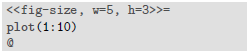
\includegraphics[scale=2]{Aliases2} 
		\label{fig:Aliases2}
\end{figure}

Lo anterior es equivalente a:

\begin{figure}[ht] 
	\centering
		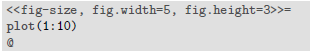
\includegraphics[scale=1.6]{Aliases3} 
		\label{fig:Aliases3}
\end{figure}

\newpage 
\subsection{Option Templates}

Una plantilla es un conjunto de opciones:
		
\begin{figure}[ht] 
	\centering
		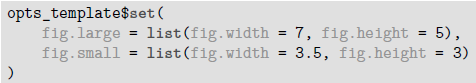
\includegraphics[scale=0.8]{Templates1}
		\label{fig:Templates1}
\end{figure}

Después de creada la plantilla, podemos simplemente usar el nombre asignado:

\begin{figure}[ht] 
	\centering
		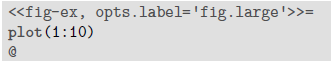
\includegraphics[scale=1.2]{Templates2} 
		\label{fig:Templates2}
\end{figure}

Lo anterior es equivalente a:

\begin{figure}[ht] 
	\centering
		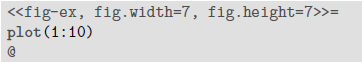
\includegraphics[scale=1.1]{Templates3} 
		\label{fig:Templates3}
\end{figure}

\newpage
\subsection{Code in Appendix}

A veces no queremos mostrar los trozos de código en el cuerpo del informe:
		
\begin{figure}[ht] 
	\centering
		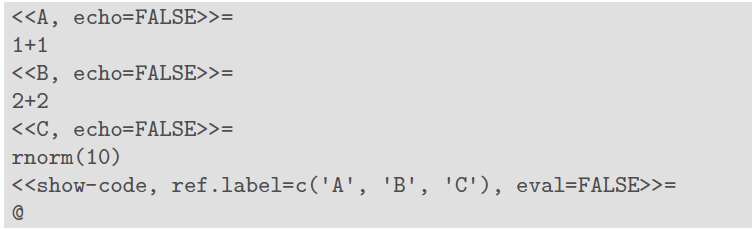
\includegraphics[scale=0.7]{Appendix1}
		\label{fig:Appendix1}
\end{figure}

Si se tienen muchos chunks en un documento, se puede hacer uso de:

\begin{figure}[ht] 
	\centering
		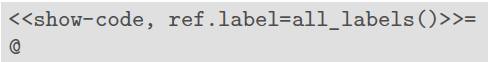
\includegraphics[scale=1]{Appendix2} 
		\label{fig:Appendix2}
\end{figure}

\subsection{Local R Options}

R.options permite tomar una lista de R por un código chunk:
		
\begin{figure}[ht] 
	\centering
		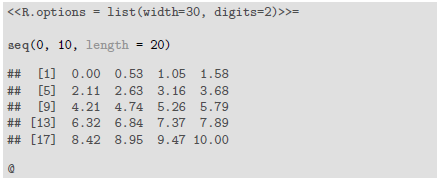
\includegraphics[scale=1.1]{Options1}
		\label{fig:Appendix1}
\end{figure}

\newpage
\section{Package Options}

Para ver más información respecto a los chuck en un código fuente, se puede activar el modo detallado por medio del comando:

\begin{figure}[ht] 
	\centering
		
\includegraphics[scale=1.8]{Package1}
		\label{fig:Package1}
\end{figure}

root.dir se puede utilizar para establecer el directorio de trabajo en el código chunk:

\begin{figure}[ht] 
	\centering
		
\includegraphics[scale=1.3]{Package2} 
		\label{fig:Package2}
\end{figure}

Para los chuck que no están etiquetados:

\begin{figure}[ht] 
	\centering
		
\includegraphics[scale=1.3]{Package3} 
		\label{fig:Package3}
\end{figure}
	
\newpage	
\section{Typesetting}	

\subsection{Output Width}

Cuando vemos que el código fuente o la salida de texto es demasiado amplia, podemos utilizar una opción de menor anchura:

\begin{figure}[ht] 
	\centering
		
\includegraphics[scale=1.8]{Width1}
		\label{fig:Width1}
\end{figure}

Sin embargo, existen casos donde la cadena de caracteres es demasiado larga en el código fuente:

\begin{figure}[ht] 
	\centering
		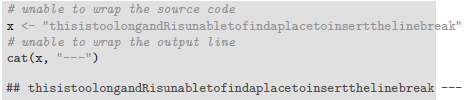
\includegraphics[scale=1.1]{Width2} 
		\label{fig:Width2}
\end{figure}

Es posible dividirla en pedazos más pequeños de forma manual y unirla nuevamente como se muestra a continuación:

\begin{figure}[ht] 
	\centering
		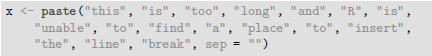
\includegraphics[scale=1.2]{Width3} 
		\label{fig:Width3}
\end{figure}

\newpage
\subsection{Box Padding}

Si sentimos que el relleno por defecto de la caja es demasiado ajustado, se puede restablecer la longitud:

\begin{figure}[ht] 
	\centering
		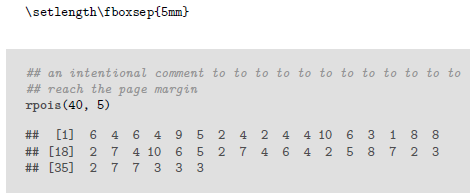
\includegraphics[scale=0.8]{Padding1}
		\label{fig:Padding1}
\end{figure}

Se puede definir la misma clase en CSS de la siguiente forma:

\begin{figure}[ht] 
	\centering
		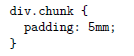
\includegraphics[scale=1.2]{Padding2} 
		\label{fig:Padding2}
\end{figure}
	
\subsection{Beamer}

Ejemplo de uso de knitr en diapositiva beamer:

\begin{figure}[ht] 
	\centering
		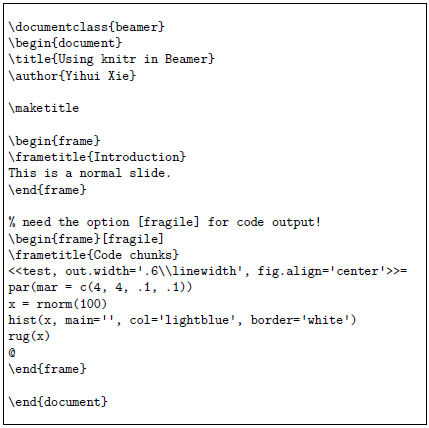
\includegraphics[scale=0.9]{Beamer1}
		\label{fig:Padding1}
\end{figure}

\newpage
Ejemplo de diapositiva con beamer:

\begin{figure}[ht] 
	\centering
		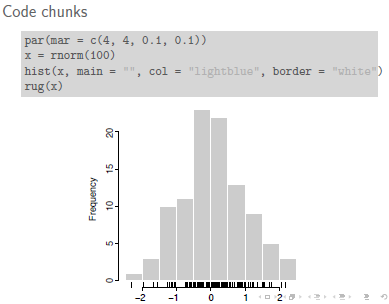
\includegraphics[scale=1.2]{Beamer2} 
		\label{fig:Padding2}
\end{figure}

\subsection{Suppress Long Output}

Omitir partes del libro, debido a que los resultados son muy largos:

\begin{figure}[ht] 
	\centering
		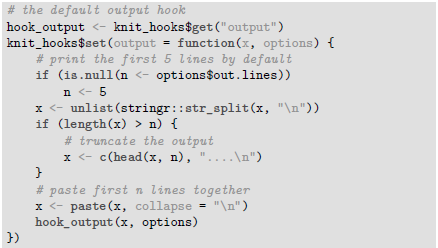
\includegraphics[scale=1.1]{Suppress1}
		\label{fig:Suppress1}
\end{figure}

\newpage
La idea básica de que la regla definida anteriormente es:

\begin{figure}[ht] 
	\centering
		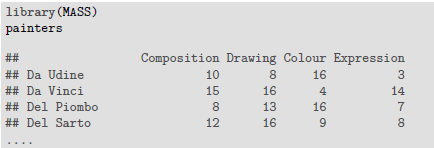
\includegraphics[scale=1.1]{Suppress2} 
		\label{fig:Suppress2}
\end{figure}

\section{Utilities}
\subsection{R Package Citation}

Por defecto se recoge los paquetes cargados en la sesión actual de R y extrae su información de la cita:

\begin{figure}[ht] 
	\centering
		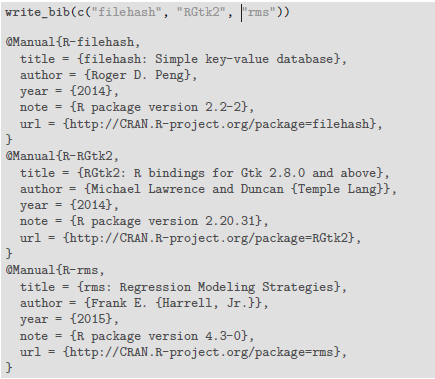
\includegraphics[scale=1]{Citation}
		\label{fig:Citation}
\end{figure}

Si el archivo principal el chunk se escribe de la siguiente forma:

\begin{figure}[ht] 
	\centering
		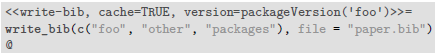
\includegraphics[scale=1.1]{Citation2} 
		\label{fig:Citation2}
\end{figure}

\newpage	
\section{Debugging}

Cuando se produce un error que no se observa claramente en la pantalla, podemos utilizar herramientas de depuración comunes, tales como traceback () (para ver el paso a paso que ha conducido al error), debug () o browser ().

\section{Multilingual Support}
		
Si el documento de origen no se ha codificado con la codificación nativa del sistema actual, tendremos que especificar manualmente su codificación mediante el argumento de codificación en:

\begin{figure}[ht] 
	\centering
		
\includegraphics[scale=1.6]{Support}
		\label{fig:Support}
\end{figure}

\section{Bibliografía}	

\bibliographystyle{apalike}						% Estilo de la bibliografía o referencias
\bibliography{biblio}							% Se muestra desde el fichero .bbl
\nocite{*}

\end{document}
